%!TEX program = xelatex

\documentclass[11pt,titlepage]{report}
%!TEX root = main.tex

\usepackage[T1]{fontenc}
\usepackage{lmodern}
\usepackage[svgnames]{xcolor}
\usepackage{fontspec} % XeLaTeX required!
\usepackage{graphicx}
\usepackage{circuitikz}
\usepackage{tikz}
\usepackage{pifont}
\usepackage[some]{background}
\usepackage{xltxtra} 
\usepackage{setspace}
\usepackage[absolute]{textpos}
\usepackage[latin1]{inputenc}
\usepackage[english]{babel}
\usepackage{graphicx}
\usepackage{wrapfig}
\usepackage{fullpage}
\usepackage[margin=1in]{geometry}
\usepackage{float}
\usepackage{url}
\usepackage{multicol}
\usepackage{hyperref}
\usepackage{titlepic}
\usepackage{standalone}
\usepackage{siunitx}
\usepackage{booktabs}
\usepackage{amsmath}
\usepackage{unicode-math}
\usepackage{verbatim}
\usepackage{enumitem}
\usepackage{listings}
\usepackage{multirow}
\usepackage{pgfplots}
\pgfplotsset{compat=1.8}
\usepackage{caption} 
\usepackage[parfill]{parskip}
\usepackage{import}
\usepackage[backend=bibtexu,texencoding=utf8,bibencoding=utf8,style=ieee,sortlocale=en_GB,language=auto]{biblatex}
\usepackage[strict,autostyle]{csquotes}
\usepackage[final]{pdfpages}
\usepackage{subcaption}
\usepackage{ifplatform}
%\captionsetup[table]{skip=10pt}


% Fix for includepdf bug in Mac OS X
\newcommand{\insertpdfpath}[1]{
	\ifwindows
	\newcommand{\insertpdf}[2]{\includepdf[pages=##1]{##2}}
	\else
	\newcommand{\insertpdf}[2]{\includepdf[pages=##1]{#1/##2}}
	\fi
}

%set fonts
\setmainfont[Ligatures=TeX]{Myriad Pro}
\setmathfont{Asana Math}
\setmonofont{Lucida Console}

\usepackage{titlesec, color}
\renewcommand{\familydefault}{\sfdefault} %set font family
\renewcommand{\arraystretch}{1.2} %set table vertical spacing
\setlength\parindent{0pt} %no paragraph indent
\hypersetup{ %setup hyperlinks
    colorlinks,
    citecolor=black,
    filecolor=black,
    linkcolor=black,
    urlcolor=black
}

%redesign chapter headings
\definecolor{gray75}{gray}{0.75}
\newcommand{\chapternumber}{\thechapter}
\newcommand{\hsp}{\hspace{20pt}}
\titleformat{\chapter}[hang]{\Huge\bfseries}{\chapternumber\hsp\textcolor{gray75}{|}\hsp}{0pt}{\Huge\bfseries}

%Redefine appendix headers
\renewcommand{\appendixname}{Appendix}
\renewcommand{\appendixtocname}{Appendices}
\renewcommand{\appendixpagename}{Appendices}

%For code listings
\definecolor{black}{rgb}{0,0,0}
\definecolor{browntags}{rgb}{0.65,0.1,0.1}
\definecolor{bluestrings}{rgb}{0,0,1}
\definecolor{graycomments}{rgb}{0.4,0.4,0.4}
\definecolor{redkeywords}{rgb}{1,0,0}
\definecolor{bluekeywords}{rgb}{0.13,0.13,0.8}
\definecolor{greencomments}{rgb}{0,0.5,0}
\definecolor{redstrings}{rgb}{0.9,0,0}
\definecolor{purpleidentifiers}{rgb}{0.01,0,0.01}


\lstdefinestyle{csharp}{
language=[Sharp]C,
showspaces=false,
showtabs=false,
breaklines=true,
showstringspaces=false,
breakatwhitespace=true,
escapeinside={(*@}{@*)},
columns=fullflexible,
commentstyle=\color{greencomments},
keywordstyle=\color{bluekeywords}\bfseries,
stringstyle=\color{redstrings},
identifierstyle=\color{purpleidentifiers},
basicstyle=\ttfamily\small}

\lstdefinestyle{c}{
language=C,
showspaces=false,
showtabs=false,
breaklines=true,
showstringspaces=false,
breakatwhitespace=true,
escapeinside={(*@}{@*)},
columns=fullflexible,
commentstyle=\color{greencomments},
keywordstyle=\color{bluekeywords}\bfseries,
stringstyle=\color{redstrings},
identifierstyle=\color{purpleidentifiers},
}

\lstdefinestyle{matlab}{
language=Matlab,
showspaces=false,
showtabs=false,
breaklines=true,
showstringspaces=false,
breakatwhitespace=true,
escapeinside={(*@}{@*)},
columns=fullflexible,
commentstyle=\color{greencomments},
keywordstyle=\color{bluekeywords}\bfseries,
stringstyle=\color{redstrings},
identifierstyle=\color{purpleidentifiers}
}

\lstdefinestyle{vhdl}{
language=VHDL,
showspaces=false,
showtabs=false,
breaklines=true,
showstringspaces=false,
breakatwhitespace=true,
escapeinside={(*@}{@*)},
columns=fullflexible,
commentstyle=\color{greencomments},
keywordstyle=\color{bluekeywords}\bfseries,
stringstyle=\color{redstrings},
identifierstyle=\color{purpleidentifiers}
}

\lstdefinestyle{xaml}{
language=XML,
showspaces=false,
showtabs=false,
breaklines=true,
showstringspaces=false,
breakatwhitespace=true,
escapeinside={(*@}{@*)},
columns=fullflexible,
commentstyle=\color{greencomments},
keywordstyle=\color{redkeywords},
stringstyle=\color{bluestrings},
tagstyle=\color{browntags},
morestring=[b]",
  morecomment=[s]{<?}{?>},
  morekeywords={xmlns,version,typex:AsyncRecords,x:Arguments,x:Boolean,x:Byte,x:Char,x:Class,x:ClassAttributes,x:ClassModifier,x:Code,x:ConnectionId,x:Decimal,x:Double,x:FactoryMethod,x:FieldModifier,x:Int16,x:Int32,x:Int64,x:Key,x:Members,x:Name,x:Object,x:Property,x:Shared,x:Single,x:String,x:Subclass,x:SynchronousMode,x:TimeSpan,x:TypeArguments,x:Uid,x:Uri,x:XData,Grid.Column,Grid.ColumnSpan,Click,ClipToBounds,Content,DropDownOpened,FontSize,Foreground,Header,Height,HorizontalAlignment,HorizontalContentAlignment,IsCancel,IsDefault,IsEnabled,IsSelected,Margin,MinHeight,MinWidth,Padding,SnapsToDevicePixels,Target,TextWrapping,Title,VerticalAlignment,VerticalContentAlignment,Width,WindowStartupLocation,Binding,Mode,OneWay,xmlns:x}
}

\lstdefinestyle{matlab}{
language=Matlab,
showspaces=false,
showtabs=false,
breaklines=true,
showstringspaces=false,
breakatwhitespace=true,
escapeinside={(*@}{@*)},
columns=fullflexible,
commentstyle=\color{greencomments},
keywordstyle=\color{bluekeywords}\bfseries,
stringstyle=\color{purpleidentifiers},
identifierstyle=\color{purpleidentifiers}
}

%defaults
\lstset{
basicstyle=\ttfamily\small,
extendedchars=false,
numbers=left,
numberstyle=\ttfamily\tiny,
stepnumber=1,
tabsize=4,
numbersep=5pt
}
\addbibresource{../../library/bibliography.bib}

\begin{document}

\chapter{Assignment 2}
\section{Calculation}
By using the online calculator located on \url{http://deepfriedneon.com/tesla_f_calcspiral.html}, we obtained acceptable inductances for our coils at the coil parameters as given in Table~\ref{tab:ass2-coil-params-calc}. Target parameters were an inner diameter of \SI{50}{mm} for both coils and inductances of \SI{22}{\micro H} for the secondary coil and \SI{100}{\micro H} for the primary coil. The diameter of the given Litz-wire is \SI{1.8}{mm} and we estimated an average wire spacing of \SI{0.5}{mm} between each winding.

\begin{table}[H]
	\centering
	\caption{Calculated coil parameters}
	\label{tab:ass2-coil-params-calc}
	\begin{tabular}{c c c c c}
		\hline\hline
		Coil & Windings & Inductance & Outer diameter & Total wire length \\
		\hline
		Primary & \num{30} & \SI{101.6}{\micro H} & \SI{188}{mm} & \SI{11.2}{m} \\
		Secondary & \num{15} & \SI{22}{\micro H} & \SI{119}{mm} & \SI{4}{m} \\
		\hline
		\end{tabular}
\end{table}

\section{Measurements}
After winding these coils we obtained the following inductances for the individual coils using an LCR-meter:

\begin{table}[H]
	\centering
	\caption{Measured coil parameters}
	\label{tab:ass2-coil-params-meas}
	\begin{tabular}{c c c}
		\hline\hline
		Coil & Inductance & DC-resistance \\
		\hline
		Primary & \SI{94.5}{\micro H} & \SI{250}{m\ohm} \\
		Secondary & \SI{25.2}{\micro H} & \SI{65}{m\ohm} \\
		\hline
		\end{tabular}
\end{table}

Then, we calculated the coils' mutual inductance and coupling factor via the ostrich approach as given in the Student Manual. \cite{epo4-manual}
This meant measuring the inductance of both of the coils while connected in \textit{series-aiding} and \textit{series-opposing} at a varying distance between the coils. The results are shown in Table~\ref{tab:ass2-coil-mutual}.

\begin{table}[H]
	\centering
	\caption{Mutual inductance and coupling factor at varying distance}
	\label{tab:ass2-coil-mutual}
	\begin{tabular}{c c c c c}
		\hline\hline
		Distance & Aiding inductance & Opposing inductance & Mutual inductance & Coupling factor \\
		\hline
		\SI{0}{cm} & \SI{184.3}{\micro H} & \SI{58.6}{\micro H} & \SI{314.2}{\micro H} & 0.64 \\
		\SI{2}{cm} & \SI{151.5}{\micro H} & \SI{86.8}{\micro H} & \SI{161.8}{\micro H} & 0.33 \\
		\SI{4}{cm} & \SI{135.6}{\micro H} & \SI{100.0}{\micro H} & \SI{88.9}{\micro H} & 0.18 \\
		\SI{6}{cm} & \SI{127.5}{\micro H} & \SI{107.0}{\micro H} & \SI{51.2}{\micro H} & 0.11 \\
		\hline
		\end{tabular}
\end{table}

\begin{figure}[H]
	\begin{center}
		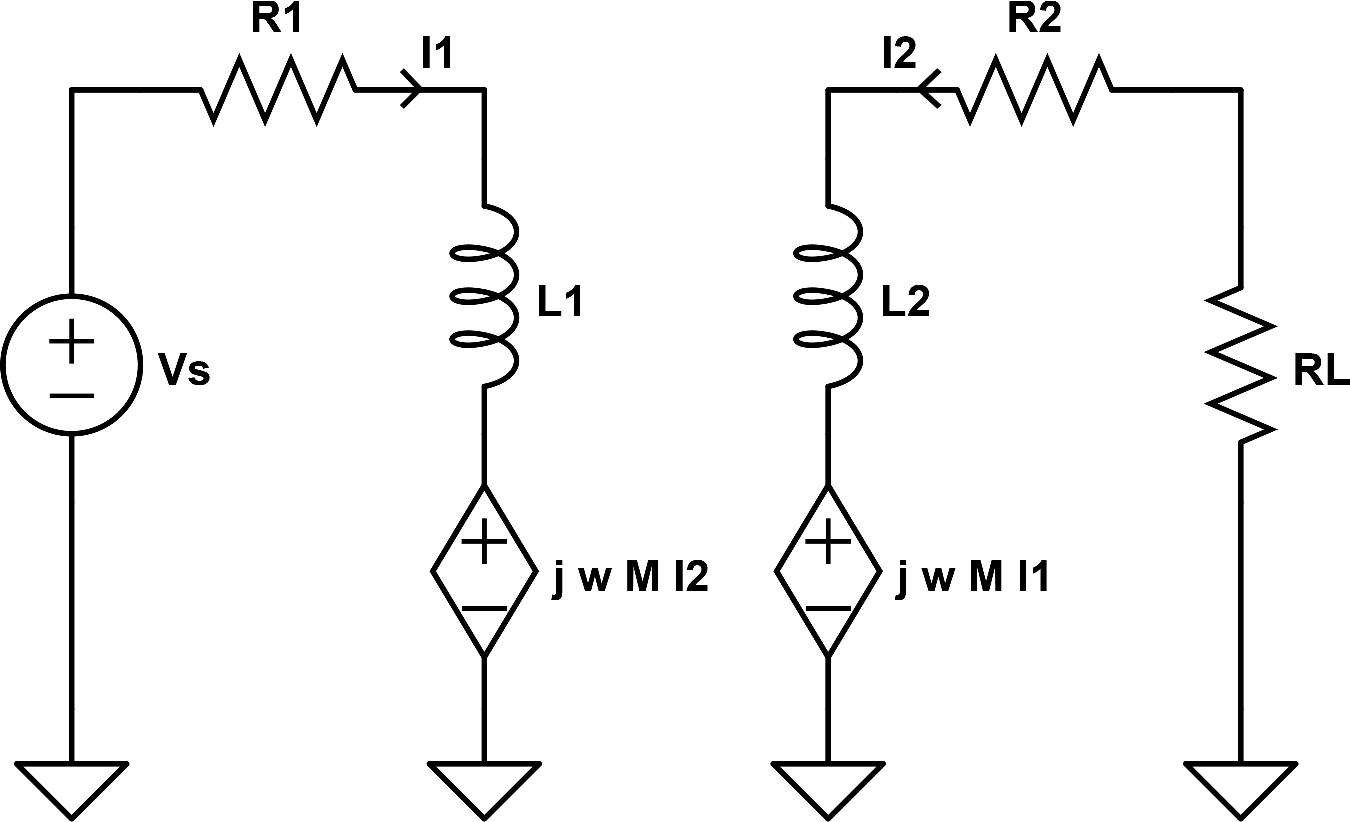
\includegraphics[width=0.6\linewidth]{resource/cpt-equivalent-circuit-uncompensated-rc.pdf}
	\end{center}
	\caption{Equivalent circuit}
	\label{fig:ass2-eq-circ}
\end{figure}

By making use of the equivalent circuit shown in Figure~\ref{fig:ass2-eq-circ} we were able to approximate the power transfer to the load. The equivalent circuit translated to a mathematical relationship given by

\begin{equation}
	\mathbf{\vec{I}} \mathbf{Z}=
	\begin{bmatrix}
		I_{source} \\
		I_{load}
	\end{bmatrix}
	\begin{bmatrix}
		R_1 + j \omega L_1 & j \omega M \\
		j \omega M & R_2 + j \omega L_2 + R_L
	\end{bmatrix}
	= \mathbf{\vec{V}} =
	\begin{bmatrix}
		V_{source} \\
		0
	\end{bmatrix} .
\end{equation}

Here the internal resistances of the coils are denoted by $R_1$ and $R_2$, the mutual inductance by $M$, the inductances by $L_1$ and $L_2$, the voltage source current by $I_{source}$ (denoted in Figure \ref{fig:ass2-eq-circ} by I1) and the load current by $I_{load}$ (denoted in Figure~\ref{fig:ass2-eq-circ} by I2). By using this relationship, we tried to approximate the power transfer characterics. The calculated values are given in Table~\ref{tab:ass2-power-sim}.

\begin{table}[H]
	\centering
	\caption{Power transfer simulations}
	\label{tab:ass2-power-sim}
	\begin{tabular}{c c c c c c c}
		\hline\hline
		Distance & Source voltage & Source current & Source power & Load voltage & Load power & Efficiency \\
		\hline
		\SI{0}{cm} & \SI{20}{V} & \SI{0.1210}{A} & \SI{2.42}{W} & \SI{4.87}{V} & \SI{2.31}{W} & \SI{96}{\percent} \\
		\SI{2}{cm} & \SI{20}{V} & \SI{0.0216}{A} & \SI{0.43}{W} & \SI{2.00}{V} & \SI{0.39}{W} & \SI{90}{\percent} \\
		\SI{4}{cm} & \SI{20}{V} & \SI{0.0069}{A} & \SI{0.13}{W} & \SI{1.04}{V} & \SI{0.11}{W} & \SI{77}{\percent} \\
		\SI{6}{cm} & \SI{20}{V} & \SI{0.0032}{A} & \SI{0.06}{W} & \SI{0.59}{V} & \SI{0.03}{W} & \SI{53}{\percent} \\
		\hline
		\end{tabular}
\end{table}

Our equivalent circuit only incorporates the losses of the internal resistances of the coils. We therefore expect the calculated efficiency and source power and consequently current to be inaccurate. Finally, we performed some measurements on the entire converter, including coils, to see how much power could be delivered to a \SI{10.08}{\ohm} load, with a distance of \SI{2}{cm} between the coils.

\begin{table}[H]
	\centering
	\caption{Power transfer measurements}
	\label{tab:ass2-power}
	\begin{tabular}{c c c c c c c}
		\hline\hline
		Distance & Source voltage & Source current & Source power & Load voltage & Load power & Efficiency \\
		\hline
		\SI{2}{cm} & \SI{19.998}{V} & \SI{0.0835}{A} & \SI{1.67}{W} & \SI{2.02}{V} & \SI{0.405}{W} & \SI{24.2}{\percent} \\
		\hline
		\end{tabular}
\end{table}

As expected, the effiency and source power and current do not match the calculated values. However, the transferred power does match the result of the simulation.

\section{Questions}
\begin{enumerate}
\item
The open and short circuit test is not well suited for the air core transformer, because that method depends on the coupling factor being very high and thus leakage flux being really low. For a ferrite-core transformer this assumption may hold, but for an air core transformer it does not, since the coupling factor decreases very fast, as the distance between the coils increases (this can be seen in Table~\ref{tab:ass2-coil-mutual}).

\item
To determine the mutual inductance of two coils, one can use the series-opposing and series-aiding method. This method makes use of the fact in both a series-aiding and series-opposing configuration, the influence of the inductance of the coils in the total inductance, that means also incorporating the mutual inductance, is the same. Thus, by substracting the measured values of the total inductance in a series aiding and series opposing configuration, one is able to substract the value of the mutual inductance because the influence of the inductances of the two coils is filtered out. However, the mutual inductance and the inductance of the two coils is heavily influenced by external factors. This should be kept in mind. 

\item
As the distance increases, the coupling factor $k$ decreases. Because the magnetising inductance $M$ is given by $k \sqrt{L_1 L_2}$, the magnetising inductance thus also decreases. Consequently, the leakage inductances $L_{L1}$ and $L_{L2}$ increase, because they are given by $L_{Li}=(1-k) L_{i}$. This result can also be obtained by arguing that the leakage flux increases by increasing the distance between the coils. An increase in leakage flux corresponds with an increase of $L_{L1}$ and a decrease of $L_{M}$.

\item
As shown in Table~\ref{tab:ass2-power}, the power transfer of the transformer is very low. This is due to the low coupling factor, especially at higher distances between the two coils.
\end{enumerate}
\end{document}